\section{Scan}
\label{sec:scan}

The third basic algorithm is the scan algorithm.
The scan algorithm is able to produce the cumulative operation of all previous array ellements given location.
Either exclusive or inclusive such as illustrated in \cref{tab:scan example}.
To compute the scan the algorithm takes an array, a binary and associative operator, and an identity element.
If the operator is add, the scan algorithm computes the running sum of the input.
The identity element is 0 for addition as shown in the ouput (excl.) from \cref{tab:scan example}.

\begin{table}[htb]
  \centering
  \begin{tabular}{r | c c c c}
    \toprule
    input & 1 & 2 & 3 & 4 \\
    operator & \multicolumn{4}{c}{$\mathtt{+}$} \\
    output (incl.) & 1 & 3 & 6 & 10 \\
    output (excl.) & 0 & 1 & 3 & 6 \\
    \bottomrule
  \end{tabular}
  \caption{Sum scan example}
  \label{tab:scan example}
\end{table}
    
A serial implementation of an inclusive sum scan is presented in \cref{lst:scan seq}.
The serial implementation follows a dynamic programming scheme where it utilizes the previously computed results to generate the next element in the output.

If the scan was to be exclusive the inclusive result would need to be shifted by one and have its first element as the identity element.
\begin{lstlisting}[caption={Serial scan}, label={lst:scan seq}]
void scan(int *h_int, int *h_out, int SIZE) {
  h_out[0] = h_in[0];
  for (int l = 1; l < SIZE; ++l)
    h_out[l] = h_out[l-1] + h_in[l];
}
\end{lstlisting}

The workload and amount of steps for the serial implementation can be expressed as follows.

\subsection{Hillis and Steele Inclusive Scan}
\label{sec:hillis and steele scan}

In this section we have provided an implementation and analysis of the Hillis and Steel inclusive scan.
The algorithm is illustrated in \cref{fig:hillis steele scan}

\begin{figure}[htb]
  \centering
  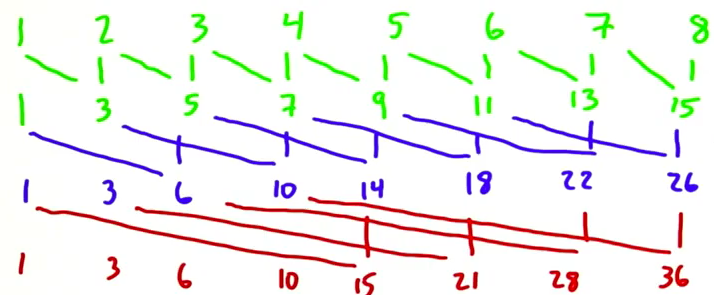
\includegraphics[width=.7\textwidth]{images/hillis-steele-scan.png}
  \caption{Hillis and Steele inclusive sum scan illustration}
  \label{fig:hillis steele scan}
\end{figure}

The algorithm utilizes the same type of dynammic programming scheme from the serial implementation though it is not as efficient.

The algorithm uses ``steps'' (not to be confused with the steps used in the algorithmic analysis) starting with step=0.
On the $i$th step, each element adds itself to the neighbour $2^i$ to the left.

Given an array where $n=ARRAY\_SIZE$ and a reduction of $2^i$ at every level of the algorithm the tree gets a height of $\mathrm{log}_2(n)$ amount of work$n \mathrm{log}_2(n)$ .


\begin{equation*}
work load = O(n \mathrm{log}_2(n))
\#steps = O(\mathrm{log}_2(n))
\end{equation*}

As of implementation details we need synchronization between each iteration of $O(lgn)$ scan tree.
To implement this synchronization we have the kernel only performing a single operation per element in the array.
To handle the height of the array we use a kernel wrapper to secure synchronization between blocks.

We present the kernel for this implementation in \cref{lst:scan par}.
Each thread calculates its position in the grid and block, and returns if it is out of bounds.
Otherwise, we make sure to add the correct element in the input or 0 if it is out of bounds.

\begin{lstlisting}[caption={Hillis and Steele scan kernel}, label={lst:scan par}]
__global__
void scan_kernel(int *d_out, int *d_in, int step, int SIZE) {
  int mid = threadIdx.x + blockDim.x * blockIdx.x;
  if (mid >= SIZE) return;

  int toAdd  = ( ((mid - step) < 0) ? 0 : d_in[mid - step] );
  d_out[mid] = d_in[mid] + toAdd;
}
\end{lstlisting}

The wrapper is shown in \cref{lst:scan wrapper}.
The wrapper secures synchronization between the different steps in the algorithm and controls the steps to be taken by the kernels by doubling the step size after each layer.
We use a temporary variable holder so we do not store values in the input array.

\begin{lstlisting}[caption={Hillis and Steele scan kernel wrapper}, label={lst:scan wrapper}]
void scan_kernel_wrapper(int *d_out, const int *d_in, int SIZE, 
                         unsigned int BYTES, int BLOCK_SIZE) {
  for (int step = 1; step < SIZE; step *= 2) {
    scan_kernel<<<GRID_SIZE,BLOCK_SIZE>>>(d_out, d_tmp, step, SIZE);
    cudaMemcpy(d_tmp, d_out, BYTES, cudaMemcpyDeviceToDevice);
  }
}
\end{lstlisting}

\Cref{fig:scan plot} presents the scan algorithm's run time development.
Noticeable is that the Hillis and Steele scan does not perform significantly better than the serial at high values.
As the algorithm grows in logarithmic complexity the workload become approximately $28$ larger at $n=2^{29}$.
Given the higher asymptotic runtime we cannot assume that the Hillis \& Steel algorithm will scale efficiently even though it is parallelizable.
However, at smaller problems we found that the Hillis \& Steele algorithm performed superior to the serial algorithm such as shown with $n = 2^{19}$ in \cref{tab:cpu vs hillis steele}.
We futher elaborated the asymptotic relationship of the Hillis \& Steele scan in \cref{sec:workload and step size}

\begin{table}[htb]
  \centering
  \begin{tabular}{c r | r r r r}
    \toprule
    device & algorithm & time in ms & speed-up & bandwidth usage & usage percentage\\
    \midrule
    CPU & serial  & 4.42 &  &  &  \\
    GPGPU & Hillis \& Steele & 1.57 & x2.81 & 72.13 GB/s & 25.01\% \\
    \bottomrule
  \end{tabular}
  \caption{Serial vs. Hillis \& Steel}
  \label{tab:cpu vs hillis steele}
\end{table}

\begin{figure}[htb]
  \centering
  \begin{tikzpicture}
  \begin{axis}[
    ymajorgrids,
    xmajorgrids,
    ylabel={Time (ms)},
    xlabel={Array size},
    xmode=log,
    log basis x={2},
    legend style={
      at={(0.05,0.95)},
      anchor=north west,
      column sep=1ex
     },
     no markers,
     very thick 
   ]

    \addplot table [x=x, y=parallel] {data/scan.csv};
    \addlegendentry{parallel};
    \addplot+[dashed] table [x=x, y=sequential] {data/scan.csv};
    \addlegendentry{sequential};
  \end{axis}
\end{tikzpicture}

  \caption{Runtime development of the scan algorithms}
  \label{fig:scan plot}
\end{figure}%
